\documentclass[aspectratio=169,11pt]{beamer}
\usepackage{booktabs}
\usepackage{tikz}
\usetikzlibrary{arrows.meta,positioning,fit,backgrounds}
\usepackage{graphicx}
\graphicspath{{../writeup/figures/}}

% Numbers generated from training/out and study/out (see training/make_figures.py)
\newcommand{\nTrain}{3300}
\newcommand{\nTest}{2200}
\newcommand{\geoR}{0.804}
\newcommand{\geoMAE}{0.314}
\newcommand{\geoRMSE}{0.404}
\newcommand{\cnnR}{0.914}
\newcommand{\cnnMAE}{0.210}
\newcommand{\cnnRMSE}{0.278}
\newcommand{\fusedR}{0.920}
\newcommand{\fusedMAE}{0.204}
\newcommand{\fusedRMSE}{0.268}
\newcommand{\sexAcc}{99.1}
\newcommand{\pslMAE}{0.29}
\newcommand{\tierExact}{62.4}
\newcommand{\tierWithinOne}{98.1}
\newcommand{\wCnn}{0.95}
\newcommand{\wGeo}{0.13}
\newcommand{\scoreMean}{2.99}
\newcommand{\scoreStd}{0.69}
\newcommand{\bestValR}{0.915}
\newcommand{\topMetric}{Jaw width : face length}
\newcommand{\topMetricR}{-0.51}
\newcommand{\nFeatures}{143}
\newcommand{\nGroups}{14}
\newcommand{\nGeometry}{58}
\newcommand{\nShape}{14}
\newcommand{\nPixel}{20}
\newcommand{\nExpression}{51}
\newcommand{\origFifteenR}{0.675}
\newcommand{\freeR}{0.820}
\newcommand{\cantTiltR}{0.00}

\newcommand{\studyPending}{}
\newcommand{\logsPending}{}


\definecolor{mgbg}{HTML}{07070B}
\definecolor{panel}{HTML}{101017}
\definecolor{mgfg}{HTML}{ECECF1}
\definecolor{muted}{HTML}{8B8B9A}
\definecolor{lime}{HTML}{C8FF3D}
\definecolor{rose}{HTML}{FF5C7A}
\definecolor{cyan}{HTML}{5EE6FF}
\newcommand{\pending}[1]{\textcolor{rose}{\textbf{[#1]}}}
\newcommand{\studyval}[1]{\ifdefined\studyPending\pending{run study}\else#1\fi}

\setbeamercolor{background canvas}{bg=mgbg}
\setbeamercolor{normal text}{fg=mgfg}
\setbeamercolor{frametitle}{fg=mgfg}
\setbeamercolor{structure}{fg=lime}
\setbeamercolor{itemize item}{fg=lime}
\setbeamercolor{alerted text}{fg=lime}
\setbeamerfont{frametitle}{series=\bfseries,size=\Large}
\setbeamertemplate{navigation symbols}{}
\setbeamertemplate{itemize items}[circle]
\setbeamertemplate{footline}{\hfill\textcolor{muted}{\scriptsize MOGSCAN \quad \insertframenumber\quad}\vspace{2mm}}
\newcommand{\stat}[2]{\begin{minipage}[t]{0.3\textwidth}\centering{\fontsize{26}{30}\selectfont\bfseries\textcolor{lime}{#1}}\\[1mm]\small\textcolor{muted}{#2}\end{minipage}}

\begin{document}

% 1 ------------------------------------------------------------------------------------------------
\begin{frame}[plain]
\vfill
\centering
{\fontsize{54}{60}\selectfont\bfseries MOG\textcolor{lime}{SCAN}}\\[4mm]
{\Large real-time $\cdot$ multi-person $\cdot$ explainable PSL}\\[10mm]
\textcolor{muted}{Ben Blair \quad$\cdot$\quad Cyril Sokolov}\\[1mm]
\textcolor{muted}{\small AI Final Project --- Startup / Product Track --- Dec 2, 2026}
\vfill
\end{frame}

% 2 ------------------------------------------------------------------------------------------------
\begin{frame}{People want to know where they stand, and \emph{why}}
\vspace{2mm}
\begin{center}
\stat{7M+}{Umax downloads,\\ $\sim$\$500K / month (mid-2024)}\hfill
\stat{Twitch}{Omoggle went viral on xQc,\\ Asmongold streams (2026)}\hfill
\stat{\$4--10}{per \emph{week} for selfie\\ face-rating subscriptions}
\end{center}
\vspace{6mm}
But every product we tested:
\begin{itemize}
  \item rates \textbf{one face at a time}: one selfie, or Omoggle's 1v1
  \item gives a \textbf{number without a reason} you can check
  \item \textbf{uploads your face} to a server
  \item has \textbf{never shown} that its score matches what real people think
\end{itemize}
\end{frame}

% 3 ------------------------------------------------------------------------------------------------
\begin{frame}{MogScan: everyone in frame, scored live, with receipts}
\begin{columns}[c]
\column{0.62\textwidth}
\IfFileExists{../writeup/figures/hero.png}{\includegraphics[width=\linewidth]{hero.png}}{%
  \fcolorbox{muted}{panel}{\parbox[c][4.6cm][c]{0.95\linewidth}{\centering\pending{Snapshot of 2--3 people\\ save as writeup/figures/hero.png}}}}
\column{0.38\textwidth}
\begin{itemize}\setlength\itemsep{2mm}
  \item Any \textbf{USB webcam}, up to \textbf{6 people}
  \item \textbf{PSL 1--8} + tier (LTN \dots\ HTN, Chadlite, Chad)
  \item Top \textbf{strengths \& weaknesses} with measured values
  \item \textbf{Mog battle} leaderboard
  \item 100\% \textbf{on-device}
\end{itemize}
\end{columns}
\end{frame}

% 4 ------------------------------------------------------------------------------------------------
\begin{frame}[plain]
\vfill\centering
{\fontsize{60}{66}\selectfont\bfseries\textcolor{lime}{LIVE DEMO}}\\[6mm]
\textcolor{muted}{solo scan $\rightarrow$ turn your head $\rightarrow$ group scan $\rightarrow$ mog battle $\rightarrow$ brutal mode}
\vfill
\end{frame}

% 5 ------------------------------------------------------------------------------------------------
\begin{frame}{How it works}
\centering
\resizebox{\textwidth}{!}{%
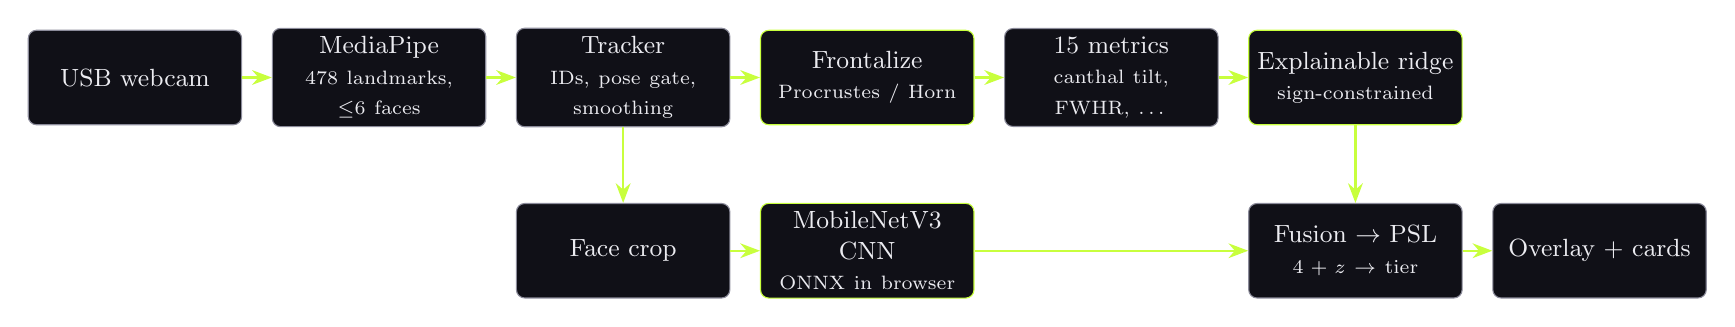
\begin{tikzpicture}[
  box/.style={draw=muted, fill=panel, text=mgfg, rounded corners=3pt, align=center, font=\small,
              minimum height=12mm, text width=25mm, inner sep=3pt},
  hi/.style={box, draw=lime},
  arr/.style={-{Stealth[length=2.5mm]}, thick, draw=lime},
]
\node[box] (cam) at (0,0) {USB webcam};
\node[box] (mp)  at (3.1,0) {MediaPipe\\\scriptsize 478 landmarks, $\le$6 faces};
\node[box] (trk) at (6.2,0) {Tracker\\\scriptsize IDs, pose gate, smoothing};
\node[hi]  (fr)  at (9.3,0) {Frontalize\\\scriptsize Procrustes / Horn};
\node[box] (met) at (12.4,0) {15 metrics\\\scriptsize canthal tilt, FWHR, \dots};
\node[hi]  (geo) at (15.5,0) {Explainable ridge\\\scriptsize sign-constrained};
\node[box] (crop) at (6.2,-2.2) {Face crop};
\node[hi]  (cnn)  at (9.3,-2.2) {MobileNetV3 CNN\\\scriptsize ONNX in browser};
\node[box] (fuse) at (15.5,-2.2) {Fusion $\rightarrow$ PSL\\\scriptsize $4 + z$ $\rightarrow$ tier};
\node[box] (ui)   at (18.6,-2.2) {Overlay + cards};
\draw[arr] (cam)--(mp); \draw[arr] (mp)--(trk); \draw[arr] (trk)--(fr); \draw[arr] (fr)--(met); \draw[arr] (met)--(geo);
\draw[arr] (trk)--(crop); \draw[arr] (crop)--(cnn); \draw[arr] (cnn)--(fuse); \draw[arr] (geo)--(fuse); \draw[arr] (fuse)--(ui);
\end{tikzpicture}}
\vspace{5mm}
\begin{columns}[t]
\column{0.33\textwidth}\small\textcolor{lime}{\textbf{Frontalize}}\\ removes head turn: the symmetry metric was $r=0.97$ with yaw before this
\column{0.33\textwidth}\small\textcolor{lime}{\textbf{Sign-constrained ridge}}\\ explanations can't contradict the data (e.g.\ FWHR sign flip)
\column{0.33\textwidth}\small\textcolor{lime}{\textbf{Trained on 5,500 faces}}\\ rated by 60 people (SCUT-FBP5500), and it runs in a browser tab
\end{columns}
\end{frame}

% 6 ------------------------------------------------------------------------------------------------
\begin{frame}{Does it agree with real people?}
\begin{columns}[c]
\column{0.5\textwidth}
\small
\begin{tabular}{@{}lc@{}}
\toprule
Model (official 60/40 split) & Pearson $r$ \\
\midrule
\textcolor{muted}{AlexNet (SCUT paper)} & \textcolor{muted}{0.830} \\
\textcolor{muted}{ResNet-18 (SCUT paper)} & \textcolor{muted}{0.851} \\
\textcolor{muted}{ResNeXt-50 (SCUT paper)} & \textcolor{muted}{0.878} \\
\midrule
Ours: geometry only & \geoR \\
Ours: CNN & \cnnR \\
\textbf{Ours: fused (live app)} & \textbf{\textcolor{lime}{\fusedR}} \\
\bottomrule
\end{tabular}\\[4mm]
\begin{itemize}
  \item PSL error \pslMAE\ points; tier within one step \tierWithinOne\%
  \item Sex head \sexAcc\% accurate (users can correct it)
\end{itemize}
\column{0.5\textwidth}
\centering
\colorbox{white}{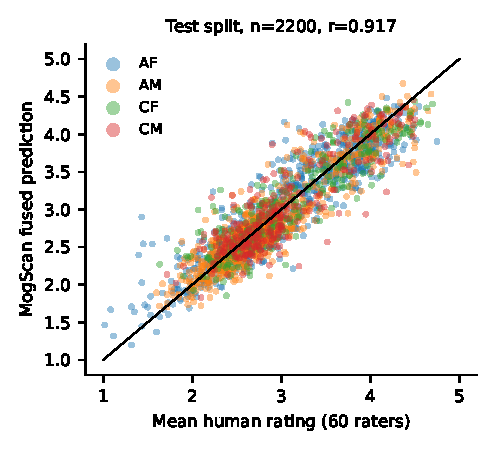
\includegraphics[width=0.88\linewidth]{scatter.pdf}}
\end{columns}
\end{frame}

% 7 ------------------------------------------------------------------------------------------------
\begin{frame}{Do looksmax rules hold up? Not all of them.}
\begin{columns}[c]
\column{0.45\textwidth}
\centering
\colorbox{white}{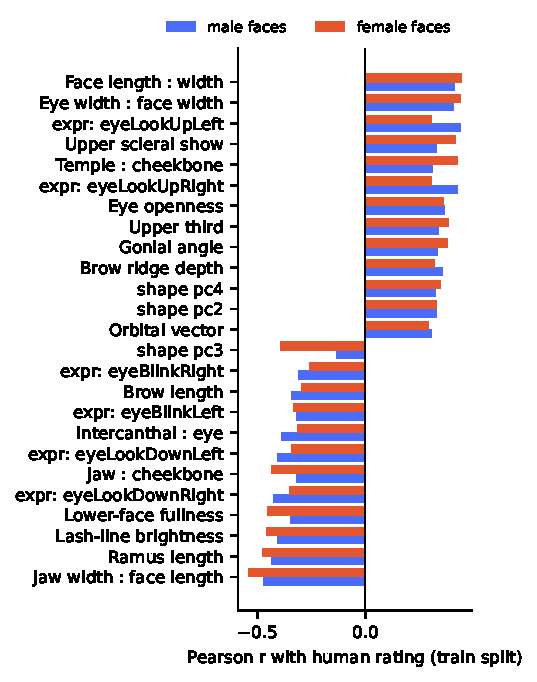
\includegraphics[width=0.92\linewidth]{metric_corr.pdf}}
\column{0.55\textwidth}
\begin{itemize}\setlength\itemsep{2mm}
  \item \textbf{Canthal tilt}: $r\approx0.00$ once head pose is removed. The earlier $+0.28$ came from pose
  \item \textbf{``Hunter eyes''}: more \emph{open} eyes were rated higher
  \item \textbf{Wide jaw / high FWHR}: \emph{narrower}, V-shaped lower faces were rated higher
  \item \textbf{Chin\,:\,philtrum} and eye spacing do match community advice
\end{itemize}
\vspace{2mm}
\small\textcolor{muted}{So MogScan shows the data-derived target \emph{and} the community range.}
\end{columns}
\end{frame}

% 8 ------------------------------------------------------------------------------------------------
\begin{frame}{Fairness check}
\centering
\begin{tabular}{@{}lcccc@{}}
\toprule
Group & $n$ & $r$ & MAE & Signed bias \\
\midrule
\csname @@input\endcsname ../writeup/generated/bias_table.tex
\bottomrule
\end{tabular}\\[6mm]
\begin{itemize}
  \item Errors and bias are similar across the four groups in the data
  \item \textbf{But}: the dataset only has Asian and Caucasian faces, so other groups are \textbf{unvalidated}
  \item \#1 priority before any commercial launch: diverse, licensed rating data
\end{itemize}
\end{frame}

% 9 ------------------------------------------------------------------------------------------------
\ifdefined\studyPending
\begin{frame}{Traction: user study}
\vfill\centering\pending{Run study/protocol.md, then make\_figures.py. This slide fills in automatically.}\vfill
\end{frame}
\else
\begin{frame}{Traction: user study}
\begin{center}
\stat{\susMean}{System Usability Scale\\(n = \studyN)}\hfill
\stat{\npsScore}{Net Promoter Score}\hfill
\stat{\payPct\%}{would pay for Pro}
\end{center}
\vspace{4mm}
\begin{columns}[c]
\column{0.55\textwidth}
\colorbox{white}{\includegraphics[width=0.95\linewidth]{survey_likert.pdf}}
\column{0.45\textwidth}\small
\agreeGroup\% said group mode was fun\\[1mm]
\agreeFeatures\% found the feature list useful\\[1mm]
\agreePrivacy\% were reassured by on-device processing\\[3mm]
\textcolor{muted}{Quotes: add 1--2 from study/out/open\_ended.md}
\end{columns}
\end{frame}
\fi

% 10 -----------------------------------------------------------------------------------------------
\begin{frame}{Competition}
\footnotesize
\begin{tabular}{@{}lccccc@{}}
\toprule
 & Omoggle & UMAX/LooksMax & PSL apps & Qoves & \textcolor{lime}{\textbf{MogScan}} \\
\midrule
Live webcam & \checkmark & -- & -- & -- & \textcolor{lime}{\checkmark} \\
Multi-person & 1v1 & -- & -- & -- & \textcolor{lime}{up to 6} \\
Per-feature measurements & -- & categories & categories & report & \textcolor{lime}{15 metrics} \\
Validated vs.\ humans & -- & -- & -- & -- & \textcolor{lime}{$r=\fusedR$} \\
On-device & claimed & -- & -- & -- & \textcolor{lime}{\checkmark} \\
Price & free & \$4--10/wk & sub & \$20--200 & \textcolor{lime}{free; \$4.99/mo} \\
\bottomrule
\end{tabular}\\[6mm]
\textbf{What we know that they don't:} \emph{explanations are the product}, and they only build trust if the
measurements agree with real ratings and survive head movement.
\end{frame}

% 11 -----------------------------------------------------------------------------------------------
\begin{frame}{Business model}
\begin{columns}[t]
\column{0.33\textwidth}
\textcolor{lime}{\textbf{Free web app}}\\[1mm]\small
Live scanning and mog battles. This is the acquisition channel and is easy to share as a link.
\column{0.33\textwidth}
\textcolor{lime}{\textbf{Pro --- \$4.99 / mo}}\\[1mm]\small
History, progress tracking, side-profile scan, evidence-based glow-up plan.
Cheaper than incumbents' \emph{weekly} price.
\column{0.33\textwidth}
\textcolor{lime}{\textbf{Creator --- \$9.99 / mo}}\\[1mm]\small
OBS overlay for Twitch/Kick ``mog battle'' streams, with branding and leaderboards.
\end{columns}
\vspace{8mm}
\centering\textcolor{muted}{Inference runs on the user's device, so marginal compute cost is close to \$0.}
\end{frame}

% 12 -----------------------------------------------------------------------------------------------
\begin{frame}{Responsible by design}
\begin{itemize}\setlength\itemsep{2mm}
  \item 18+ and consent screen; only scan people who agree
  \item Nothing uploaded or stored; study logs are numbers only
  \item ``Kind'' wording by default; the score is framed as \emph{one panel's judgement}, not your worth
  \item We measure wellbeing in the study (``felt worse about my looks'')
  \item Known limits: two ethnic groups, binary sex labels, webcam domain shift, non-commercial dataset license
\end{itemize}
\end{frame}

% 13 -----------------------------------------------------------------------------------------------
\begin{frame}{What's next}
\begin{columns}[c]
\column{0.6\textwidth}
\begin{itemize}\setlength\itemsep{2mm}
  \item Diverse, licensed rating dataset $\rightarrow$ retrain and publish subgroup error
  \item Side-profile scan: gonial angle, chin projection, E-line
  \item OBS streamer overlay with battle ELO
  \item Progress tracking + glow-up plan
  \item Grad-CAM heatmaps and a WebGPU backend
\end{itemize}
\column{0.4\textwidth}
\centering
\IfFileExists{qr.png}{\colorbox{white}{\includegraphics[width=0.7\linewidth]{qr.png}}\\[1mm]\small Try it live}{%
\fcolorbox{muted}{panel}{\parbox[c][3.5cm][c]{0.8\linewidth}{\centering\small\pending{QR code to deployed URL\\ slides/qr.png}}}}
\end{columns}
\end{frame}

\begin{frame}[plain]
\vfill\centering
{\fontsize{44}{50}\selectfont\bfseries MOG\textcolor{lime}{SCAN}}\\[5mm]
{\large Thank you. Questions?}\\[3mm]
\textcolor{muted}{Ben Blair \quad$\cdot$\quad Cyril Sokolov}
\vfill
\end{frame}

\end{document}
